\begin{figure}[htbp]
	\centering

    \subfloat[Box plot, \acs{SCT}, $\sigma_n=1068$ Pa, P=0.8.]{
	  \includegraphics[width=.75\columnwidth]{images/145BoxSCT1068p08sinterfine}
	  \label{fig:145BoxSCT1068p08sinterfine}  }
	 
    \subfloat[Box plot, \acs{SCT}, $\sigma_n=1068$ Pa, P=1.0.]{
	  \includegraphics[width=.75\columnwidth]{images/148BoxSCT1068p10sinterfine}
	  \label{fig:147BoxSCT1068p10sinterfine}  } 
	  
    \subfloat[Box plot, \acs{SCT}, $\sigma_n=1068$ Pa, P=1.2.]{
	  \includegraphics[width=.75\columnwidth]{images/147BoxSCT1068p12sinterfine}
	  \label{fig:148BoxSCT1068p12sinterfine}  } 	  
	  

 % \hfill\null
  \caption[SCT box plots 1]{SCT box
  plots for sinter fine, $\sigma_n=1068$ Pa.}
  \label{fig:146boxplotsct1068}
\end{figure}

% \begin{figure}%[!h] 
% \centering 
% 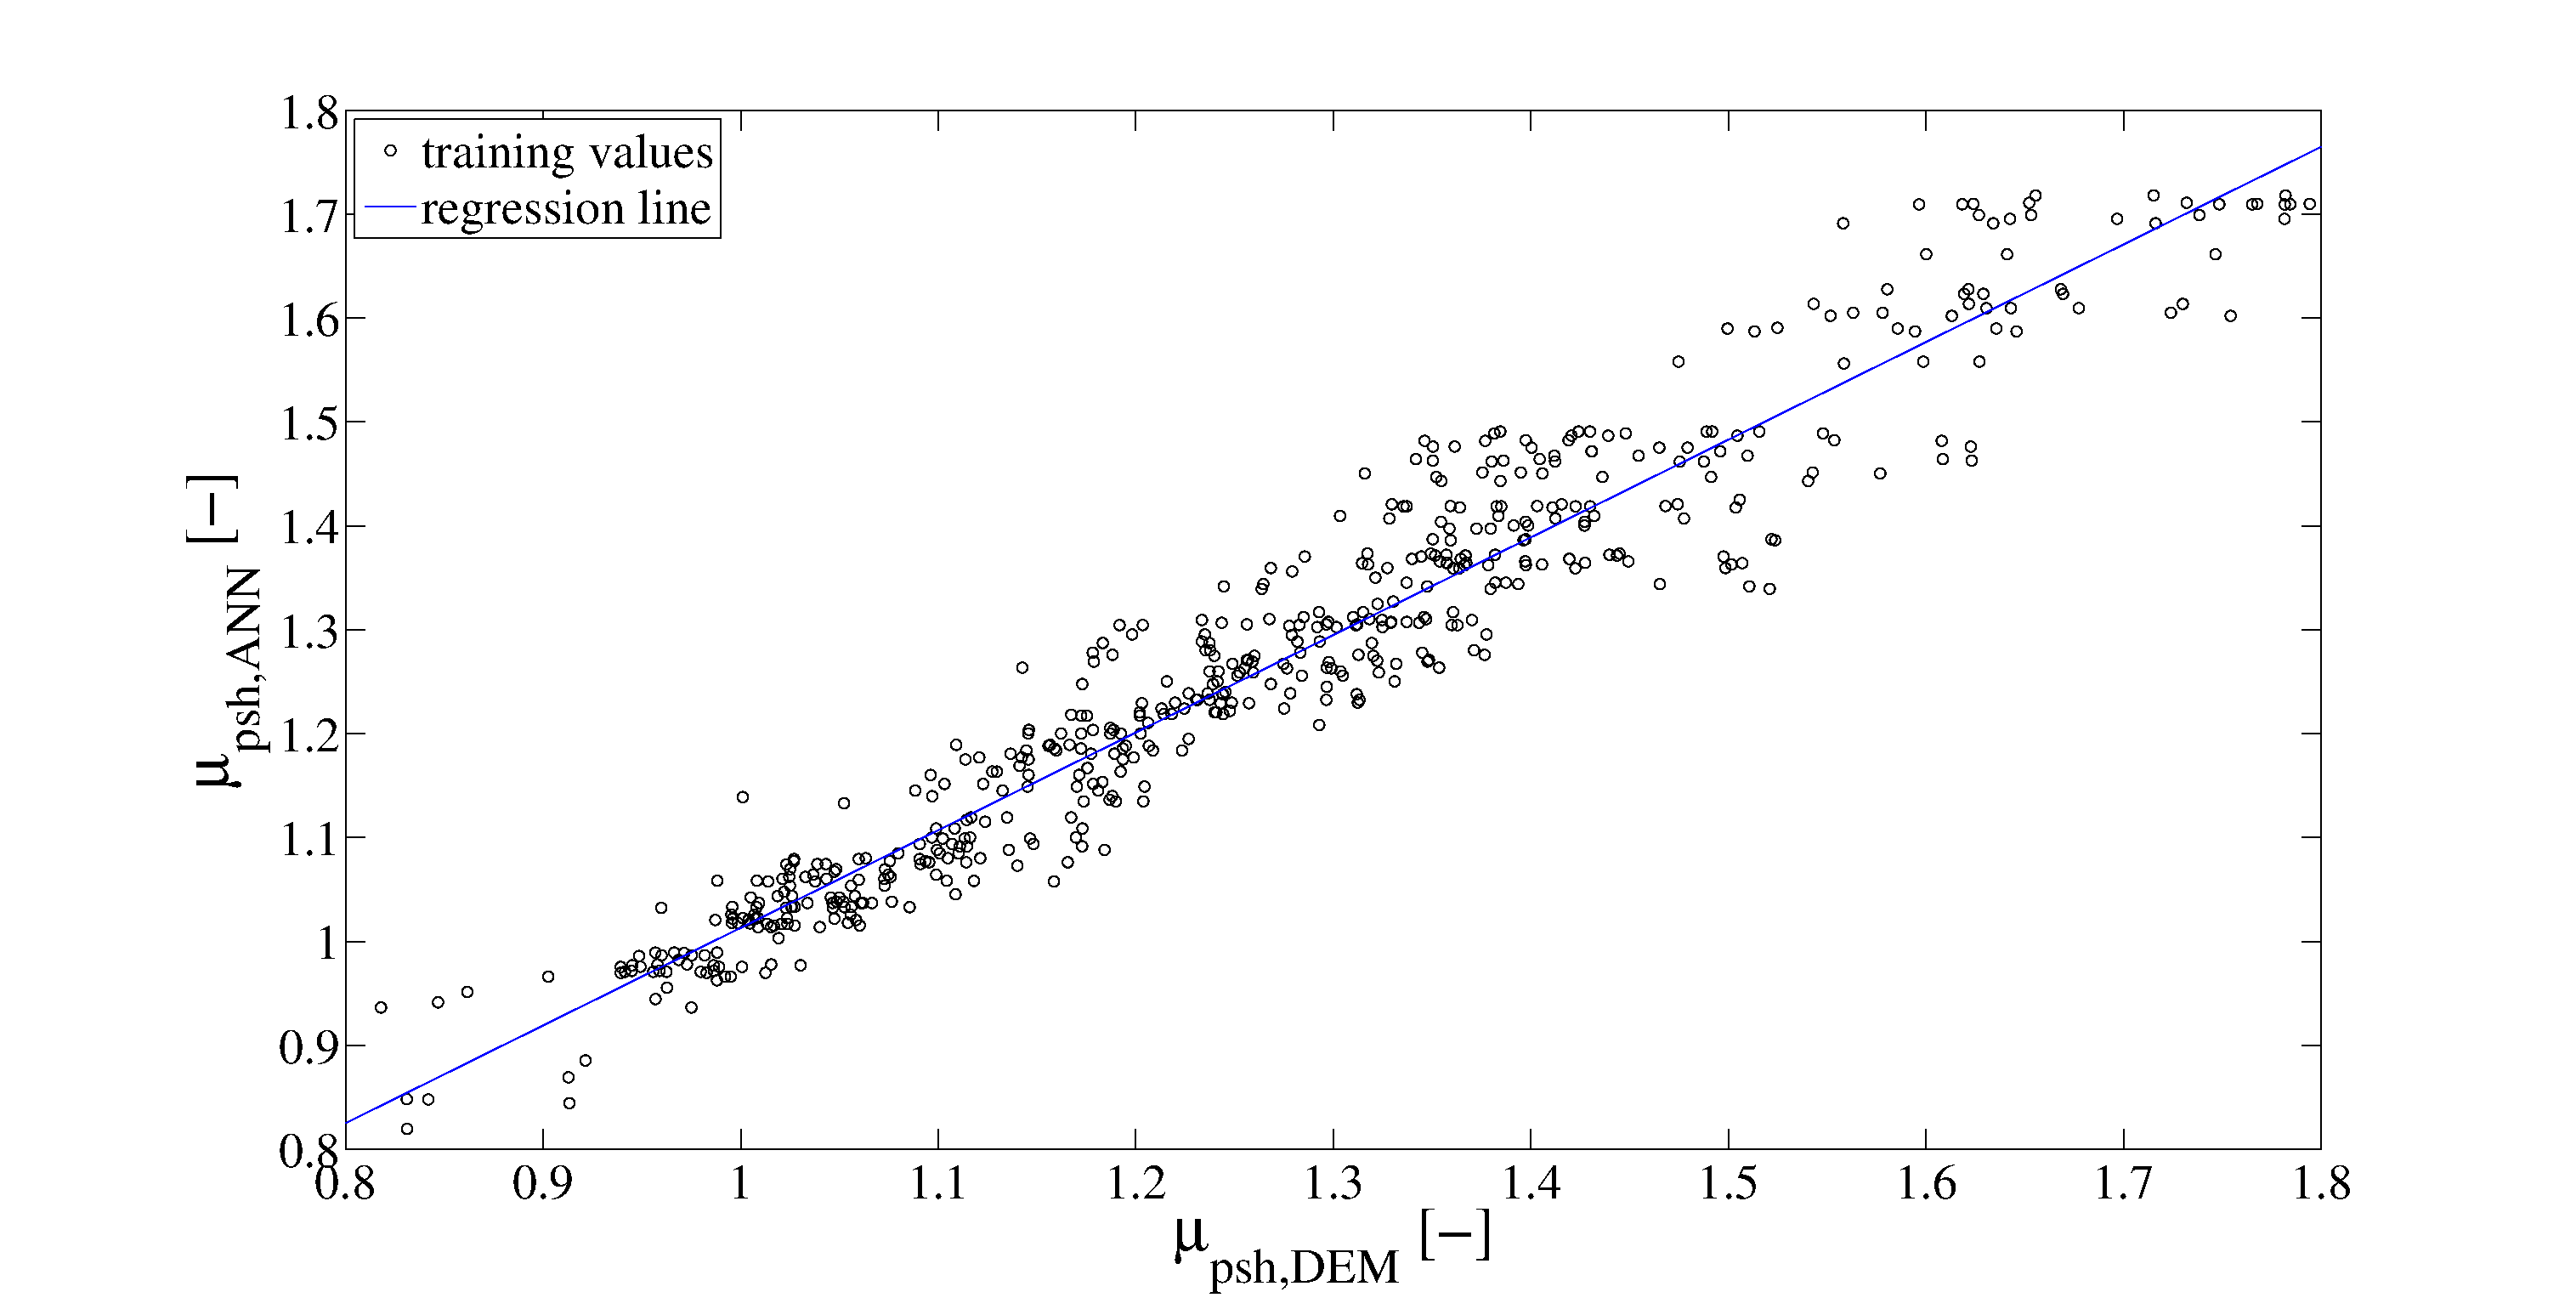
\includegraphics[width=.80\columnwidth]{images/022regression.eps}
% %[width=.48\textwidth]
% \caption[Comparison between prediction of the trained ANN and full DEM
% simulation]{Comparison between prediction of the trained Artificial Neural
% Network (\acs{ANN}) and 546 
% \wrong{write down all the simulations performed at the end.}
% full DEM simulations of the coefficient of pre-shear
% (\acs{mupsh}).}
% \label{fig:022regression} 
% \end{figure}